\documentclass[../main.tex]{subfiles} % ~1400 Worte

\begin{document}

\subsection{Benutzeranforderungen als Use Cases} % Lauritz

Bei der Entwicklung von Softwareprojekten, wie der Webanwendung `ShroomScout', ist die sorgfältige Definition von
Benutzeranforderungen ein entscheidender Schritt. Eine bewährte Strategie zur Strukturierung und Priorisierung dieser
Anforderungen ist die Erstellung von Use Cases. Use Cases beschreiben typische Interaktionen zwischen dem Nutzer und
dem System und dienen dazu, klare und nachvollziehbare Anforderungen zu formulieren. Im Folgenden werden die zentralen
Use Cases für `ShroomScout' detailliert beschrieben, um die grundlegenden Benutzeranforderungen zu veranschaulichen
(siehe Abbildung~\ref{fig:UseCase_Diagramm}).

\begin{figure}[ht]
	\centering
	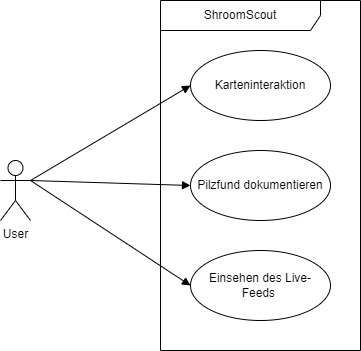
\includegraphics[width=0.5\textwidth]{abbildungen/UseCaseDiagrammDrawio.jpg}
	\caption{Use Cases von ShroomScout.}
	\label{fig:UseCase_Diagramm}
\end{figure}

\subsubsection{Karteninteraktion}

Die Karte ist das zentrale Element von `ShroomScout' und ermöglicht es den Nutzern, bereits eingetragene Pilzfundorte
visuell zu erfassen. Nutzer können auf der Karte navigieren, indem sie hin- und herscrollen sowie hinein- und herauszoomen,
um unterschiedliche Bereiche und Detailstufen zu erkunden. Diese Funktionen sind essenziell, um die Suche nach Pilzstandorten
intuitiv und effizient zu gestalten. Bereits eingetragene Pilzfundorte sind mit einem Marker markiert und der Name des dort
gefundenen Pilzes kann durch anklicken oder hovern angezeigt werden. Die Interaktion mit der Karte ist also in Anlehnung an
andere kartenbasierte Anwendungen konzipiert, sodass Nutzer leicht den gewünschten Kartenausschnitt oder eingetragenen Pilz
finden können, was die hohe Benutzerfreundlichkeit der Anwendung ermöglicht.

\subsubsection{Pilzfund dokumentieren}

Ein weiterer zentraler Use Case ist das Eintragen eines Pilzfunds durch den Nutzer. Dieser Prozess beginnt mit dem Klick
auf die Schaltfläche `Pilz eintragen' und umfasst mehrere Schritte:

\begin{itemize}

	\item \textbf{Eingabe von Pilzname und Umgebung:}
	      Der Nutzer gibt den Namen des Pilzes ein, unterstützt durch eine automatische Vervollständigung, um Tippfehler zu
	      vermeiden und den Prozess zu beschleunigen. Zusätzlich wird die Umgebung des Pilzfunds (z.B. Wiese, Eiche) erfasst.

	\item \textbf{Anzeigen eines Bildes des Pilzes:}
	      Nach der Eingabe des Pilznamens wird automatisch ein Bild des entsprechenden Pilzes angezeigt. Dies dient der visuellen
	      Bestätigung und hilft, Verwechslungen zu vermeiden.

	\item \textbf{Markieren des Fundorts auf der Karte:}
	      Der Nutzer platziert einen Marker auf der Karte, um den genauen Fundort des Pilzes zu dokumentieren.

	\item \textbf{Finale Dokumentation:}
	      Sind alle Informationen angegeben, kann der Pilzfundort mit einem Knopf eingetragen werden. Um sicherzustellen, dass alle
	      notwendigen Eingaben getätigt worden sind, aktiviert sich dieser erst, wenn die drei oben stehenden Aktionen ausgeführt
	      worden sind. So kommt es zu keinen fehlerhaften Einträgen, was weiter zur Benutzerfreundlichkeit und Einfachheit beiträgt.

\end{itemize}

\subsubsection{Einsehen des Live-Feeds}

Der Live Feed stellt eine Auflistung der jüngsten Pilzfunde dar und wird kontinuierlich aktualisiert. Obwohl Nutzer mit dem
Live Feed nicht direkt interagieren können, dient er als wichtige Informations- und Inspirationsquelle für die Community.
Die Anzeige der neuesten Funde fördert das Gemeinschaftsgefühl und motiviert Nutzer, eigene Entdeckungen zu teilen. Obwohl der
Live Feed keine direkte Nutzerinteraktion beinhaltet, ist er ein wesentlicher Bestandteil des Nutzererlebnisses und trägt zur
Dynamik der Anwendung bei.

Zusammenfassend bilden diese Use Cases das Fundament für die Interaktion der Nutzer mit `ShroomScout' und definieren klare
Anforderungen an die Funktionalität und Benutzerfreundlichkeit der Anwendung. Durch die detaillierte Ausarbeitung dieser Use
Cases wird sichergestellt, dass die Entwicklung von `ShroomScout' den Bedürfnissen und Erwartungen der Zielgruppe entspricht
und eine intuitive, effiziente und ansprechende Benutzererfahrung bietet.

\subsection{Funktionale Anforderungen} % Tim

\subsection{Nicht-funktionale Anforderungen} % Lauritz

Neben den funktionalen Anforderungen, die spezifische Aktionen und Verhaltensweisen des Systems beschreiben, spielen
nicht-funktionale Anforderungen eine entscheidende Rolle für den Erfolg eines Softwareprojekts. Sie definieren die
Qualitätsattribute der Anwendung und beeinflussen maßgeblich die Nutzerzufriedenheit. Für die Webanwendung `ShroomScout'
lassen sich folgende nicht-funktionale Anforderungen festhalten:

\begin{itemize}

	\item \textbf{Einfachheit und Benutzerfreundlichkeit}
	      `ShroomScout' soll durch eine intuitive Bedienbarkeit bestechen. Die Anwendung muss so gestaltet sein, dass Nutzer mit
	      minimalen Aufwand und ohne Vorkenntnisse die Kernfunktionalitäten nutzen können. Dazu gehört eine klare und verständliche
	      Nutzeroberfläche, die es dem Anwender ermöglicht, ohne umständliche Navigation oder komplizierte Prozesse Pilze zu finden
	      und einzutragen.

	\item \textbf{Responsive Design}
	      Angesichts der Tatsache, dass Nutzer `ShroomScout' häufig im Freien und damit auf mobilen Geräten nutzen werden, ist ein
	      responsive Design unerlässlich. Die Anwendung muss sich automatisch an verschiedene Bildschirmgrößen und -auflösungen
	      anpassen, um auf Smartphones, Tablets und Desktop-Computern gleichermaßen gut bedienbar zu sein. Dies gewährleistet eine
	      optimale Benutzererfahrung unabhängig vom Endgerät.

	\item \textbf{Schnelle Ladezeiten}
	      Für eine positive Nutzererfahrung sind kurze Ladezeiten von großer Bedeutung. `ShroomScout' sollte so optimiert sein,
	      dass die Anwendung auch bei langsamer Internetverbindung schnell lädt. Dies ist besonders wichtig, da Nutzer die Anwendung
	      möglicherweise in Gebieten mit schlechter Netzabdeckung verwenden.

	\item \textbf{Sicherheit und Datenschutz}
	      Die Sicherheit persönlicher Daten und die Wahrung der Privatsphäre der Nutzer sind essenzielle Anforderungen. `ShroomScout'
	      muss sicherstellen, dass alle Nutzerdaten, insbesondere Standortinformationen und persönliche Informationen, gemäß den
	      geltenden Datenschutzrichtlinien behandelt und geschützt werden.

	\item \textbf{Skalierbarkeit}
	      Die Anwendung muss in der Lage sein, mit einer zunehmenden Anzahl von Nutzern und Datenmengen zu skalieren. Dies stellt
	      sicher, dass `ShroomScout' auch bei wachsender Beliebtheit und steigenden Anforderungen stabil und performant bleibt.

	\item \textbf{Barrierefreiheit}
	      `ShroomScout' sollte so gestaltet sein, dass die Anwendung auch für Menschen mit Behinderungen zugänglich ist. Dies
	      umfasst beispielsweise die Implementierung von Screenreader-Unterstützung und die Anpassung von Farbkontrasten für eine
	      bessere Lesbarkeit.

	\item \textbf{Mehrsprachigkeit}
	      Um eine breite Nutzerbasis anzusprechen und die Anwendung auch für nicht deutschsprachige Pilzsammler attraktiv zu machen,
	      sollte `ShroomScout' die Möglichkeit bieten, die Benutzeroberfläche in verschiedenen Sprachen darzustellen.

\end{itemize}

Durch die Berücksichtigung dieser nicht-funktionalen Anforderungen in der Entwicklungsphase wird sichergestellt, dass `ShroomScout'
nicht nur funktionell den Bedürfnissen der Nutzer entspricht, sondern auch in Bezug auf Qualität und Benutzerfreundlichkeit überzeugt.

\end{document}
